\documentclass{elsarticle}
% \usepackage{graphicx}
\usepackage{hyperref}
%\usepackage{multicol}
%\usepackage{footmisc}
\usepackage{amstext}
\usepackage{amsmath}
\usepackage{amssymb}
\usepackage{mathrsfs}
\usepackage{amsthm}
\usepackage[english]{babel}
%\usepackage[official,right]{eurosym}
\selectlanguage{english}
\hyphenation{ExecEngine}
\newtheorem{lemma}{Lemma}
\begin{document}
% Ampersand -----------------------------------------------------------

%\def\id#1{\text{\it #1\/}}
\newcommand{\id}[1]{\text{\it #1\/}}
\newcommand{\code}[1]{\text{\tt\small #1}}
\newcommand{\stmtText}[1]{``{\small\tt #1}''}
\newcommand{\dom}[1]{\id{dom}(#1)}
\newcommand{\cod}[1]{\id{cod}(#1)}
\renewcommand{\int}[2]{\id{inter}(#1,#2)}
\newcommand{\relsIn}[1]{\id{relsIn}(#1)}    % maps a Term to a set of Relations
\newcommand{\maintain}{\id{maint}}
\newcommand{\pop}[2]{\id{pop}_{#1}(#2)}
\newcommand{\inst}{\id{inst}}
\newcommand{\relname}[1]{\id{relname}(#1)}
\newcommand{\src}[1]{\id{src}(#1)}
\newcommand{\tgt}[1]{\id{tgt}(#1)}
\newcommand{\sat}[2]{\id{sat}_{#1}(#2)}
\newcommand{\viol}[2]{\id{viol}_{#1}(#2)}
\newcommand{\sign}[1]{\id{sign}(#1)}
\newcommand{\powerset}[1]{\cal{P}\{#1\}}
\newcommand{\theCode}{\url{http://cs.ru.nl/~B.Joosten/ampTypes/}}
\newcommand{\la}{\langle}
\newcommand{\ra}{\rangle}
\newcommand{\full}{V}
\newcommand{\declare}[3]{\id{#1}_{\pair{#2}{#3}}}
\newcommand{\subst}[3]{#3_{[#1\rightarrow #2]}}
\newcommand{\fullt}[2]{V_{\pair{#1}{#2}}}
\newcommand{\iden}{I}
\newcommand{\ident}[1]{I_{\id{#1}}}
\newcommand{\expr}[3]{(#1)_{#2\times #3}}
\newcommand{\pair}[2]{\la{#1},{#2}\ra}
\newcommand{\Pair}[2]{#1\times#2}
\newcommand{\pairs}[1]{\id{pairs}(#1)}
\newcommand{\triple}[3]{\la{#1},{#2},{#3}\ra}
\newcommand{\quadruple}[4]{\la{#1},{#2},{#3},{#4}\ra}
\newcommand{\atom}[1]{{\tt\small #1}}
\newcommand{\atoms}{\mathcal{A}}
\newcommand{\Atoms}{\mathbb{A}}
\newcommand{\concept}[1]{{\tt\small #1}}
\newcommand{\concepts}{\mathcal{C}}
\newcommand{\Concepts}{\mathbb{C}}
\newcommand{\decls}{\mathcal{D}}  %% names of relations
\newcommand{\rels}{\mathcal{R}}   %% all relations
\newcommand{\Rels}{\mathbb{R}}   %% all relations
\newcommand{\relations}{\mathcal{M}} % representing terms. M is a subset of R.
\newcommand{\triples}{\mathcal{T}}
\newcommand{\Triples}{\mathbb{T}}
\newcommand{\Triple}[3]{#1\times#2\times#3}
\newcommand{\vertices}{N}
\newcommand{\rules}{\mathcal{U}}
\newcommand{\Rules}{\mathbb{U}}
\newcommand{\specrules}{\mathcal{S}}
\newcommand{\roles}{\mathcal{O}}
\newcommand{\Events}{{\mathit E}}
\newcommand{\dataset}{\mathscr{D}}
\newcommand{\Dataset}{\mathbb{D}}
\newcommand{\schema}{\mathscr{Z}}
\newcommand{\functionality}{\mathscr{F}}
\newcommand{\select}[2]{\id{select}_{#1}\{{#2}\}}
\newcommand{\migrsys}{\mathscr{M}}
\newcommand{\infsys}{\mathscr{S}}
\newcommand{\tf}[1]{\mathscr{T}(#1)}
\newcommand{\ptf}[1]{\mathscr{T}'(#1)}
\newcommand{\ti}[1]{\mathscr{I}(#1)}
\newcommand{\tic}[1]{I_{\cal C}(#1)}
\newcommand{\relAdd}{\dagger}
\newcommand{\flip}[1]{{#1}^\smallsmile} %formerly:  {#1}^\backsim
\newcommand{\kleeneplus}[1]{{#1}^+}
\newcommand{\kleenestar}[1]{{#1}^*}
\newcommand{\cmpl}[1]{\overline{#1}}
\newcommand{\rel}{\times}
\newcommand{\compose}{;}
\newcommand{\subs}{\subseteq}%{\models}
\newcommand{\fun}{\rightarrow}
\newcommand{\isa}{\preceq}
%\newcommand{\isaClos}{\sqsubseteq}
\newcommand{\typetest}{?}
\newcommand{\meet}{\sqcap}
\newcommand{\join}{\sqcup}
\newcommand{\Meet}{\bigsqcap}
\newcommand{\Moin}{\bigsqcup} % because LaTeX has already defined command \Join.
\newcommand{\order}{\ominus}
\newcommand{\anything}{\top}
\newcommand{\nothing}{\bot}
\newcommand{\rewriteto}{\rightarrow}
\newcommand{\calc}{\implies}
\newcommand{\alland}{\bigwedge}
\newcommand{\mph}[3]{#1_{#2\times #3}}
\newcommand{\mphu}[1]{#1_{\univ\times\univ}}

%-----------------------------------------
\newcommand{\kse}{\hspace*{1.7em}}
\newcommand{\ksf}{\hspace*{1em}}
\newcommand{\ksg}{\hspace*{1em}}
\newenvironment{derivation}{\begin{tabbing}\kse \= \ksf \= \ksg \= \kill}{\end{tabbing}}
\newtheorem{definition}{Definition}
\newcommand{\term}[1]{\>\>\(#1\)\\[1ex]}
\newcommand{\rela}[2]{\>\(#1\)\>\>\{ \ #2 \ \}\\[1ex]}
\newcommand{\weg}[1]{}

\def\define#1{\label{dfn:#1}{\em #1}\index{#1}}
\def\definem#1{\label{dfn:#1}{\em #1}\index{#1}\marge{#1}}
\newcommand{\marg}[1]{\index{#1}\marge{#1}}


% TODO Algemeen:
% - type van triple-set en atom-set definieren zodat viol_u ?->P(?x?)
%   (Bas: ik heb foute types weggehaald, maar dit nog niet gedefinieerd)
% - nieuwe populatie na de disjoint union zou de populatie met ENFORCE regels toegepast moeten zijn
%  (en in het bijzonder de ISA regels)

% TODO Stef:
% - stukje literatuuronderzoek
% https://ieeexplore.ieee.org/abstract/document/7445334?casa_token=ECzi6XeV2ncAAAAA:KhWzB8XBFOUJ0C6AD-XjX_ryuA9ARvTd3gm6RR-ZNiR8sZ1858FJpQ7zKQhkAZDlv8IjPdgD
% https://ieeexplore.ieee.org/abstract/document/8549944?casa_token=9qiGqNzh2Q0AAAAA:C-cYogExB35nGxQdxLcdBh4JoLNvM0OHedAMhCbB5V4kb4_6nzHUvc23xSJbeoBu67LSiz-Y
% https://citeseerx.ist.psu.edu/viewdoc/download?doi=10.1.1.651.9298&rep=rep1&type=pdf
% https://www.scirp.org/html/4-7800724_106592.htm
% https://www.researchgate.net/profile/Ranjana-Badre/publication/318665687_GUI_for_Data_Migration_and_Query_Conversion/links/5b45bbea0f7e9b1c722386e5/GUI-for-Data-Migration-and-Query-Conversion.pdf
% https://journal3.uin-alauddin.ac.id/index.php/literatify/article/view/12567

% Bewijsverplichtingen:
% -> het migratie-systeem is typefout-vrij (opmerking: als we de type-checker buiten beschouwing willen laten, kunnen we dit niet beschrijven)
% -> het migratie-systeem is vrij van overtredingen op regels die het migratie-systeem moet bewaken
% -> het migratie-systeem bevat alle oude data, ihb nog steeds na het toepassen van de enforce regels
% -> er is een pad naar ingebruikname van het nieuwe systeem (vanaf de initiële toestand van het migratie-systeem)
% -> corollary: op het moment van ingebruikname van het nieuwe systeem, is het migratie-systeem vrij van overtredingen op regels die het nieuwe systeem moet bewaken
% -> optioneel: na een begrensd aantal 'voortgangs-stappen' kan het nieuwe systeem in gebruik genomen worden
% -> optioneel: er bestaat een migratie-systeem dat de oude functionaliteit behoudt (mogelijk uitbreid) totdat het nieuwe systeem in gebruik genomen is?

\title{Data migration under a Changing Schema}
\author[ou,ordina]{Stef Joosten\fnref{fn1}}
\ead{stef.joosten@ou.nl}
\author[umn]{Sebastiaan Joosten\fnref{fn2}}
\address[ou]{Open Universiteit Nederland, Heerlen, the Netherlands}
\address[ordina]{Ordina NV, Nieuwegein, the Netherlands}
\address[umn]{University of Minnesota, Minneapolis, USA}
\fntext[fn1]{ORCID 0000-0001-8308-0189}
\fntext[fn2]{ORCID 0000-0002-6590-6220}

\begin{abstract}
   To support incremental software development with a software generator bears the potential of saving work and decreasing the time to deploy changes.
   However, increments that change the database schema cause nontrivial data migration issues.
   The problem is how to preserve the semantics of the data as much as possible and satisfy elementary business requirements at the same time.

   To generate an information system in a non-incremental manner is already
   provided for by the Ampersand project.
   This paper is about changing an already generated system in production.
   It develops a theory for deploying an incremental change,
   making Ampersand more useful for agile software development.
   This paper proposes a migration method that features zero down-time,
   and features an undo after deployment.
   It also leaves room for the business to finish ongoing work
   after the moment the change has been deployed.
\end{abstract}

\begin{keyword}
generative software\sep incremental software development\sep data migration\sep relation algebra\sep Ampersand\sep schema change
\end{keyword}
\maketitle

\section{Introduction}
\label{sct:Introduction}
   The purpose of this work is to automate the data migrations that come with incrementally developing and deploying information systems.
   This paper proposes a theory for such data migrations in the context of generated information systems%
\footnote{In the sequel, the word ``system'' refers to the phrase ``information system''. This simplifies the language a little. }.

   This paper is founded in the belief that generating systems can prevent human programming errors, which contributes to robust software.
   Besides, information systems should be released into production in small increments.
   That yields shorter release cycles, more frequent releases, and thus a more agile software development process%
   \footnote{These effects can be measured in terms of DevOps metrics such as
   deployment frequency,
   reliability of deployments, and
   change failure rate~\cite{DevOps2021}.}.
   By installing upgrades automatically, frequently, in small increments, and without down-time,
   the users experience a system that evolves organically, without even noticing the updates.
   By automating data migrations correctly and reliably, migration engineers save effort and errors.
   As a result, they can release smaller increments more frequently, which contributes to a more agile software development process.
   Smaller and faster releases also mean a smaller difference between the existing system and the desired system.
   This yields even simpler migrations, leveraging even more frequent releases.
   
   Differences of schemas of an existing system and a desired system complicate the migration of data.
   The purpose of incremental deployment poses specific requirements to data migration,
   which sets it apart from data migrations for other purposes.
   For instance, if a data migration is done for switching to another platform or to different technology,
   e.g.~\cite{Gholami2016,Bisbal1999},
   migration engineers may deliberately avoid schema differences and functionality changes to avoid introducing new errors in an otherwise error-prone migration process.
   For the purpose of software updates, however, introducing new functionality, removing obsolete functionality, and schema differences are the very reason for deploying an increment.
   Data migration literature sometimes uses a different notion of increment.
   For example, Ataei, Khan, and Walkingshaw~\cite{Ataei2021,Walkingshaw2014} define an increment as a variation between two data structures.
   They show how to unify databases with slight variations by preserving all variations in one comprehensive database.
   In a software update, however, the variations are not preserved.
   So this notion of increment in\cite{Ataei2021} is obviously different.
   Examples like these have convinced the authors to define a new method for data migration that is specifically meant for systems in production that are
   deployed incrementally.
   
   The contribution of this paper is to derive a migration schema from two artifacts: an existing system
   (which has its own schema and dataset) and a new schema (which specifies the desired system).
   The purpose of our theory is to develop tools.
   These tools must satisfy such practical requirements as
   zero down-time updates and ways to cope with data pollution.
   Zero down-time means that all human activity for the data migration can be done without taking the system out of production.
   In practice, more frequent updates require that updates come with zero down-time.
   Any delay caused by automatically switching from the existing system to the desired is considered negligible.
   This assumes a modern deployment platform (such as Kubernetes) that updates applications with zero down-time.
   
   Our theory is based on the following assumptions and requirements:
\begin{itemize}
   \item the data migration is meant to deploy a software increment in production;
   \item the existing data set may be polluted, but it satisfies its schema;
   \item the data migration may require human interaction, which may take time;
   \item the meaning of data must be preserved;
   \item the business continues during the migration without interruption;
   \item there is a compiler to generate an information system from a given schema.
\end{itemize}
   This paper focuses on the correctness of the migration.
   Efficiency of the migration is beyond the scope.

\section{Analysis}
\label{sct:Analysis}
   The purpose of an information system is to make data meaningful to its users.
   The analysis of the problem starts with a formal definition of information systems,
   in which the schema contains all information that makes data meaningful.
   We then define a migration procedure from one information system to another,
   which preserves the meaning of the data as much as possible.

   Users have their own tasks and responsibilities
   and may work from different locations and on different moments.
   This collective use by multiple users serves a purpose which we will loosely call ``the business''.
   It is this business that depends on the semantics of the data to draw the right conclusions and carry out their tasks.
   This paper uses semantic constraints to represent this meaning.
   
   Information systems are typically used by actors (both users and computers) who are distributed and work with data all the time.
   As a consequence, the data in a system changes continually.
   In practice, actors ``talk to'' the system through an ingress mechanism, which connects each user to the right service(s).
   The ingress function is provided by the deployment platform, so it is beyond the scope of this paper.
   Also, every service runs independent of other services,
   meaning that each service can be stopped, (re)started and substituted without disrupting the other services.

   Every system contains a dataset, which represents the state of the system.
   Every service produces and consumes events that may change the state of the system.
   This state is represented in a persistent store, aka the database%
\footnote{Whether the database is local, remote, or globally distributed is immaterial for the theory in this paper.}.
   Events that the system detects may cause the state to change.
\begin{figure}[bht]
   \begin{center}
     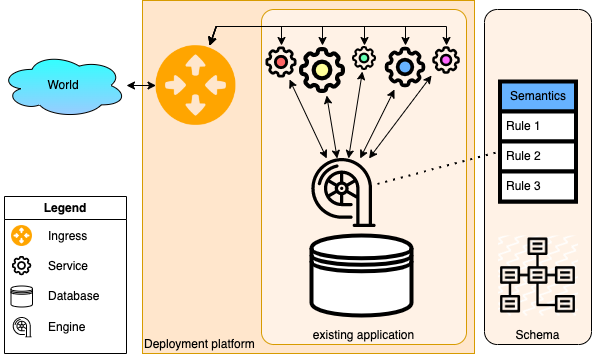
\includegraphics[scale=.45]{datamigration-Pre-migration.drawio.png}
   \end{center}
\caption{Anatomy of an information system}
\label{fig:pre-migration}
\end{figure}
   To keep our theory technology independent, datasets are assumed to contains triples.
   This makes our theory valid for any kind of database that triples can represent,
   such as SQL databases, object-oriented databases, graph databases, triple stores, and other no-SQL databases.
   The system's semantics is represented as constraints,
   which most database management systems refer to as integrity rules.
   The purpose of integrity rules is to keep the constraints they represent satisfied.

   This work uses the Ampersand compiler~\cite{Joosten-JLAMP2018} to validate the theory.
   Ampersand is a tool to generate information systems.
   It works with relations in a way similar to Alloy~\cite{Alloy2006} and allegories%
\footnote{Allegories are a specific type of categories, which the reader does not need to understand for the purpose of this paper}~\cite{Zielinski2013}.
   Each rule in Ampersand is a constraint (aka invariant), which the Ampersand run-time engine keeps satisfied as long as that rule lives%
\footnote{The dotted lines in the diagrams show which set of rules the engine keeps satisfied.}.
   So, the user spends no effort to extract constraints from specifications or (even more laborious) from code
   because all constraints are explicitly available as rules in the code.
   This, and the absence of imperative code in an Ampersand script, makes Ampersand a suitable platform to validate the theory.
   It also allows us to be explicit about ``preserving the meaning as much as possible''.
   An Ampersand script contains just enough information to generate a complete system,
   which means that a classical database schema (i.e.\ data structure plus semantics) can be extracted from the Ampersand script.
   For the purpose of this paper an Ampersand script is considered equivelant to the schema of the generated system.

   Data migration occurs when a desired system replaces an existing one,
   while preserving the meaning of the present data as much as possible~\cite{Spivak2012}.
   Just copying the set of data from the existing system to the desired system is obviously wrong if the schemas of both systems differ.

   Complications may arise as a result of data pollution,
   which may require human interventions to resolve.
   Data pollution is distinguished in the following categories:
\begin{itemize}
   \item data pollution that violates a constraint in the schema.
   \item data pollution that violates a constraint that is not in the schema.
   \item data pollution that cannot be captured in constraints on the dataset,
   such as a street address that has become obsolete because someone has moved without notification.
   \item data pollution that is a consequence of an erroneous constraint in the schema.
\end{itemize}
   The first category is about violations of constraints from the schema.
   Such violations do not occur in our theory because the existing system was generated by Ampersand,
   so the existing system has kept all constraints from the schema satisfied.
   This sets our approach apart from other approaches to formalize data migration, e.g.~\cite{Thalheim2013}.
   The second category, data pollution that is not captured by any of the constraints mentioned in the schema,
   can be dealt with by adding constraints in the desired system.
   In that case, a migration engineer must ensure that the desired system can start with data that satisfies all constraints in its schema.
   So some human intervention may be necessary in specific cases.
   The third category of pollution must be dealt with by working procedures, to prevent such pollution as much as possible.
   In some cases, constraints on data can be formulated,
   so the system can help the user and simplify (or eliminate) the corresponding working procedure.
   So, such constraints may help to move this type of pollution to one of the other categories.
   The last category of data pollution, erroneous constraints, must be fixed by replacing them by the correct constraints in the desired system.

   This illustrates that automating data migrations may require user intervention,
   either by a migration engineer or by end-users.
   In our approach, such user interventions are given some time by
   defining two distinct moments:
\begin{enumerate}
   \item the moment of transition (the MoT), i.e. the moment the desired system is made available to users;
   \item the moment of no return (the MoN), i.e. the moment that the migration cannot be undone other than by a backup-procedure%
\footnote{Backup mechanisms are outside the scope of this paper.}.
\end{enumerate}

   During the time between the MoT and MoN,
   the existing system and the desired system are kept alive, side by side, as shown in figure~\ref{fig:migration phase}.
\begin{figure}[bht]
   \begin{center}
     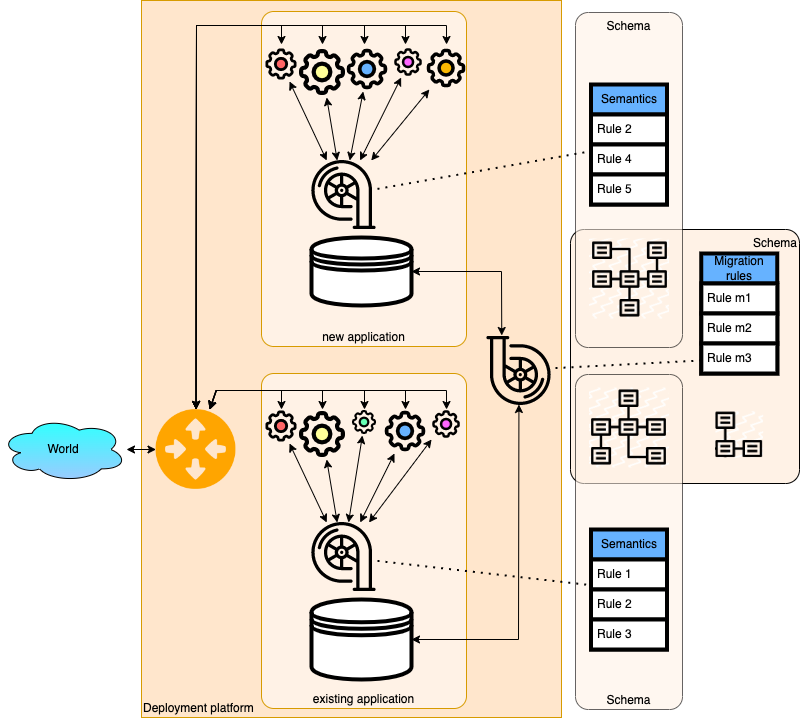
\includegraphics[scale=.35]{datamigration-Migration phase.drawio.png}
   \end{center}
\caption{Migration phase}
\label{fig:migration phase}
\end{figure}

   The migration requires a third schema, which specifies the migration itself.
   The migration schema comprises the schemas of both the existing system and the desired system.
   The rules of the migration schema will cause the right data to be copied correctly into the desired system.
   This migration schema preserves data from the existing system, it may introduce new data automatically (generated from the existing dataset),
   and it may require users to introduce new data (which will take time). 
   So the idea of a migration schema is to compute the disjoint union of the existing and the desired schemas
   and to present it to the migration engineer in the form of source code,
   so the migration engineer can change everything she wants to suit the particulars of the data migration.

%    A naive migration might proceed as follows:
%    Launch the desired system in parallel to the existing one, copy data from the existing to the desired system, and have everyone use the desired system.
%    However, numerous issues might impede that plan.
%    The following examples illustrate the practical issues that may occur:
% \begin{enumerate}
% \item Data required in the desired system is missing in the existing system.
%    There may be no way in the existing system to enter that data.
%    An example could be that every reimbursement form needs to have an address associated to it to mail the check to, but address information is not stored in the existing system:
%    The existing system required the reimbursement office to look up employee's addresses from a hand-written list they had on their desk.

%    This issue will require somebody to insert the missing addresses in the desired system.
% \item Data in the existing system is wrong but cannot be corrected there due to how the existing system was designed.
%    An example is if the existing system only allows approvals to be entered as the current user, and the CEO has always insisted that her administrative staff enters the approvals into the system for her.
%    This may result in approvals being entered as admin staff, where it was really the CEO making the approval.

%    This issue will require that the incorrect registration of staff members is corrected in the desired system.
% \item Data in the existing system does not satisfy invariants of the desired system.
%    There may be no way in the existing system of making the data satisfy those invariants.
%    We can use the same example as in the previous bullet point,
%    but add the requirement (in the desired system) that every purchase above a certain amount needs to be approved by the CEO.

%    This issue will require somebody to change the data to satisfy the broken invariants in the desired system.
% \item A way of entering data into the existing system is missing in the desired system.
%    People or automated processes might rely on these ways of entering data.
%    An example could be that when employees turned their computers on or off,
%    an ad-hoc script would automatically check them in- and out to determine the number of hours they worked.
%    A handful of employees still relies on this.

%    This issue will require that users of obsolete functionality are informed and given a way to cope with the missing functionality where appropriate.
% \item Data present in the existing system cannot be stored in the desired system.
%    An example could be that references to physical locations where original receipts are kept are stored in the existing system,
%    but the desired system relies on scans of receipts and allows the originals to be destroyed or not submitted.

%    This issue will require that the existing data is kept until the original receipts have been scanned.
% \end{enumerate}

% (@Bas, het volgende zit al in de oplossingen sfeer. Willen we dat hier al doen?)
%    To mitigate these issues, we:
   
%    \begin{enumerate}
%    \item Allow `missing' triples requirements to be ignored during migration.
%    \item Allow triples to be migrated while being marked as needing correction.
%    \item Allow invariants in the desired system to be ignored for certain triples during migration.
%    \item Allow continued use of interfaces of the existing system, data entered into the existing system via those interfaces needs to be continuously copied to the desired system.
%    \item Retain data in the existing system until it can be marked as ready to be phased out.
%    \end{enumerate}   

   During the migration phase, transactions in the existing system are allowed because the migration engine will transport them to the desired system.
   This allows the business to finish transactions in the existing system while the desired system is already up and running.
   Similarly, the existing system must execute transactions from the desired system, just in case the business calls off the migration.
   Rules in the migration system that require user interaction are given time by requiring that the migration phase ends
   only after all migration rules are at rest.
   At the MoN, the migration engineer takes down everything but the desired system,
   leaving the business with a successful migration.
\begin{figure}[bht]
   \begin{center}
     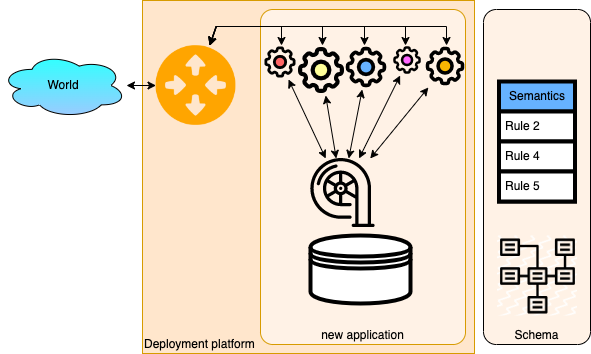
\includegraphics[scale=.35]{datamigration-Post-migration.drawio.png}
   \end{center}
\caption{The system after the data migration}
\label{fig:post-migration}
\end{figure}

   In the following section introduces the definitions required to migrate data from one system to another.

\section{Terminology}
\label{sct:Terminology}
   An {\em information system} is a combination of dataset, schema, and functionality.
   For the purpose of this paper, the functionality is ignored because it does not impact the migration.
   Section~\ref{sct:Datasets} desribes datasets. Schemas are treated in section~\ref{sct:Schemas}.
   Then section~\ref{sct:Information Systems} defines information systems.

\subsection{Datasets}
\label{sct:Datasets}
   A dataset $\dataset$ describes a set of structured data, which is typically stored persistently in a database of some kind.
   The notation $\dataset_{\infsys}$ refers to the dataset of a particular information system $\infsys$.
   The purpose of a dataset is to describe the data of a system at one point in time. 
   Before defining datasets, let us first define the constituent notions of atom, concept, specialization, relation, and triple.
   
   Atoms serve as data elements.
   Atoms are values without internal structure of interest, meant to represent atomic data elements (e.g. dates, strings, numbers, etc.) in a database.
   From a business perspective, atoms represent concrete items of the world,
   such as \atom{Peter}, \atom{1}, or \atom{the king of France}.
   By convention throughout the remainder of this paper, variables $a$, $b$, and $c$ represent \emph{atoms}.
   All atoms are taken from an infinite set called $\Atoms$.
   
   Concepts are names that group atoms of the same type.
   All concepts are taken from an infinite set $\Concepts$.
   $\Concepts$ and $\Atoms$ are disjoint.
   For example, a developer might choose to classify \atom{Peter} and \atom{Melissa} as \concept{Person},
   and \atom{074238991} as a \concept{TelephoneNumber}.
   In this example, \concept{Person} and \concept{TelephoneNumber} are concepts.
   In the sequel, variables $A$, $B$, $C$, $D$ will represent concepts.

   The relation $\inst:\Pair{\Atoms}{\Concepts}$ relates atoms to concepts.
   The expression $a\inst C$ means that atom $a$ is an \emph{instance} of concept $C$.
   This relation is used in the type system, in which $\inst$ assigns one or more concepts to every atom in the dataset.

   Specialization, also known as {\em generalization} or {\em subtyping}, is a relation between concepts.
   The statement $A\isa B$ (pronounce: $A$ is a $B$) states that any instance of $A$ is an instance of $B$ as well.
\begin{equation}
   \label{eqn:specialization}
   A\isa B\ \Leftrightarrow\ \forall a: a\inst A\rightarrow a\inst B
\end{equation}
   Specialization is needed to allow statements such as: ``An employee is a person'' or ``A human is a mammal''.
   In her script, a user can declare a specialization as a pair of concepts in the relation $\isa$.
   A compiler can construct $\isa$ as the transitive, reflexive closure of all user-defined specializations.
   It must make sure that $\isa$ is antisymmetric, so that $\isa$ is a partial order of concepts.
   Specialization causes atoms to have multiple concepts of which they can be an instance.
   As a result, if an atom is an instance of concept $A$ and $A\isa B$,
   this atom has all properties that atoms of type $B$ have.

   Relations serve to organize and store data, to allow a developer to represent facts.
   In this paper, variables $r$, $s$, and $d$ represent relations.
   All relations are taken from an infinite set $\Rels$.
   $\Rels$ is disjoint from $\Concepts$ and $\Atoms$.
   Every relation $r$ has a name, a source concept, and a target concept.
   The notation $r=\declare{n}{A}{B}$ denotes that relation $r$ has name $n$, source concept $A$, and target concept $B$.
   The part $\pair{A}{B}$ is called the {\em signature} of the relation.

%    The following is for wide tables only
%    Specialization distributes in a straightforward way over signatures:
% \begin{equation}
%    \pair{A}{B}\isa\pair{C}{D}\ \Leftrightarrow\ A\isa C\ \wedge\ B\isa D
% \label{eqn:isa-signature}
% \end{equation}

   Triples serve to represent data.
   A triple\footnote{Please note that this paper uses the word {\em triple} in a more restricted way than in natural language.}
   is an element of $\Triple{\Atoms}{\Rels}{\Atoms}$.

   A dataset $\dataset$ is a tuple $\pair{\triples}{\inst}$ that satisfies:
\begin{eqnarray}
   \triple{a}{\declare{n}{A}{B}}{b}\in\triples&\Rightarrow&a\inst A\ \wedge\ b\inst B
   \label{eqn:wellTypedEdge}
\end{eqnarray}
   For example, $\triple{\text{\atom{Peter}}}{\declare{\id{phone}}{\tt Person}{\tt TelephoneNumber}}{\text{\atom{074238991}}}$ is a triple.
   Equation~\ref{eqn:wellTypedEdge} says that \atom{Peter} is an instance of {\tt Person} and \atom{074238991} is an instance of {\tt TelephoneNumber}.
   In practice, users can say that Peter has telephone number 074238991.
   So, the ``thing'' that \atom{Peter} refers to (which is Peter) has \atom{074238991} as a telephone number.
   This ``meaning from practice'' has no consequences in the formal world.
   Users are free to attach any practical meaning to a triple.

   The notations $\triples_{\dataset}$ and $\inst_{\dataset}$ are used to disambiguate $\triples$ and $\inst$ when necessary.
   Every dataset is an element of an infinite set called $\Dataset$,
   which is disjoint from $\Rels$, $\Concepts$ and $\Atoms$.
   To save writing in the sequel, the notation $a\ r\ b$ means that $\triple{a}{r}{b}\in\triples$.

   A relation $r$ can serve as a container of pairs,
   as defined by the function $\id{pop}_r:\Dataset\rightarrow\powerset{\Pair{\Atoms}{\Atoms}}$.
   It defines a set of pairs, also known as the population of $r$:
\begin{equation}
   \pop{r}{\dataset}\ =\ \{ \pair{a}{b}\mid\ \triple{a}{r}{b}\in\triples_{\dataset}\}
\label{eqn:pop-rel}
\end{equation}
   Equation~\ref{eqn:wellTypedEdge} implies that for every dataset $\dataset$:
\[\pair{a}{b}\in\pop{\declare{n}{A}{B}}{\dataset}\ \Rightarrow\ a\inst_{\dataset}A\ \wedge\ b\inst_{\dataset}B\]
   For a developer, this means that the type of an atom depends only on the relation in which it resides; not on the actual population of the database.

   Concepts too can be seen as containers of atoms,
   defined by the function $\id{pop}_C:\Dataset\rightarrow\powerset{\Atoms}$.
\begin{equation}
   \pop{C}{\dataset}\ =\ \{ x\mid\ x\ \inst_{\dataset}\ C\}
\label{eqn:pop-concept}
\end{equation}

\subsection{Schemas}
\label{sct:Schemas}
   Schemas serve to capture the semantics of an information system~\cite{Spivak2012}.
   A schema defines concepts, specializations, relations, and rules.
   A software engineer defines a schema on design time, so that semantic checks can be implemented at compile time.

   A schema $\schema$ is a tuple $\quadruple{\concepts}{\isa}{\rels}{\rules}$,
   in which $\concepts$ is a finite set of concepts,
   $\isa$ is a partial order of concepts,
   $\rels$ is a finite set of relations,
   and $\rules$ is a finite set of rules.
   Each rule in a schema serves to constrain the dataset at runtime, to ensure its semantic integrity.
   Every rule is an element of an infinite set called $\Rules$,
   which is disjoint from $\Atoms$, $\Concepts$, $\Rels$, and $\Dataset$.
   In this paper, variables $u$ and $v$ represent rules.
   The notation $\schema_{\infsys}$ refers to the schema of information system $\infsys$.
   Disambiguation sometimes requires to write $\concepts_{\schema}$, $\isa_{\schema}$, $\rels_{\schema}$, and $\rules_{\schema}$
   rather than $\concepts$, $\isa$, $\rels$, and $\rules$ respectively.
   For every rule $u$ in the schema, there is a predicate $\sat{u}{\dataset}$ that says whether or not dataset $\dataset$ satisfies rule $u$.
%  Every schema is an element of an infinite set called $\Schema$.

   A schema must ensure that triples ``make sense'' in the semantics defined by the schema.
   This means that it must satisfy the following requirements.
\begin{eqnarray}
   \declare{n}{A}{B}\in\rels&\Rightarrow&A\in\concepts\ \wedge\ B\in\concepts
   \label{eqn:relationsIntroduceConcepts}\\
   A\ \isa\ B&\Rightarrow&A\in\concepts\ \wedge\ B\in\concepts
   \label{eqn:isasIntroduceConcepts}\\
%    The following is for wide tables only
%    \pair{A}{B}\isa\pair{C}{D}\ \wedge\ \declare{n}{C}{D}\in\rels&\Rightarrow&\declare{n}{A}{B}\in\rels
%    \label{eqn:subrelations}\\
   \isa\ \text{is a partial order}
   \label{eqn:isasPartialOrder}\\
   \exists\dataset\in\Dataset-\emptyset:\ \sat{u}{\dataset}
   \label{eqn:consistentRules}
\end{eqnarray}
   Requirement~\ref{eqn:relationsIntroduceConcepts} ensures that concepts mentioned in a relation are defined in the schema.
   Requirement~\ref{eqn:isasIntroduceConcepts} ensures that the specialization relation works on concepts of $\concepts$.
%    The following is for wide tables only
%    Requirement~\ref{eqn:subrelations} ensures that all specializations of a relation exist.
   Requirement~\ref{eqn:isasPartialOrder} ensures that the specialization relation contains no cycles.
   Requirement~\ref{eqn:consistentRules} ensures that every rule is consistent.

   The type system of Ampersand~\cite{vdWoude2011} ensures that every information system it generates satisfies these requirements.
   Note that these requirements do not depend on any particular dataset,
   so they can be checked at compile time.
   This is also known as static typing,
   which has well established advantages for the software engineering process~\cite{HanenbergKRTS14,Petersen2014}.

%    For every rule $u$ in the schema, we assume there is a function $\id{viol}_u : \Dataset\rightarrow\powerset{\Pair{\Atoms}{\Atoms}}$
%    that represents the set of violations%
% \footnote{The definition of ``violation'' is not needed in this paper. We only use the absence of violations to show satisfaction of a rule.}
%    of rule $u$ in any dataset.
%    We also assume a function $\id{sign} : \Rules\rightarrow\Pair{\Concepts}{\Concepts}$
%    that represents the signature of a rule, i.e. the type of atoms in violations:
% \begin{eqnarray}
%    \sign{u}=\pair{A}{B}\ \wedge\ \pair{a}{b}\in\viol{u}{\dataset}&\Rightarrow&a\inst A\wedge b\inst B
%    \label{eqn:wellTypedEdged violations}
% \end{eqnarray}
%    To determine whether rule $u$ is satisfied in dataset $\dataset$,
%    we define $\sat{u}{\Dataset}$:
% \begin{eqnarray}
%    \sat{u}{\dataset}&\Leftrightarrow&\viol{u}{\dataset}=\emptyset
%    \label{eqn:sat}
% \end{eqnarray}
%    Violations are used to produce meaningful error messages and to trigger changes in the dataset to restore satisfaction of that rule.

\subsection{Information Systems}
\label{sct:Information Systems}
   This section defines the notion of information system.
   As before, a suffix disambiguates the elements of this definition when needed.
\begin{definition}[information system]
\label{def:information system}
\item An information system $\infsys$ is a tuple $\quadruple{\dataset}{\schema}{\roles}{\maintain}$, in which
\begin{itemize}
   \item dataset $\dataset=\pair{\triples}{\inst}$ is defined as in section~\ref{sct:Datasets};
   \item schema $\schema=\quadruple{\concepts}{\isa}{\rels}{\rules}$ is defined as in section~\ref{sct:Schemas};
   \item $\roles$ is a set of roles;
   \item ${\maintain} : \roles\times\rules$ is the maintainance relation between roles and rules.
\end{itemize}
\end{definition}
   A \define{role} is a name that identifies a group of users.
   It serves as a placeholder for a person or a machine (i.e. an actor) that works with the dataset (i.e. create, read, update, or delete triples).
   The purpose of a role is to mention an individual user (human) or an automated actor (bot) without knowing who that user is.

   The information system enforces the semantics by ensuring that the following requirements remain true at all times:
\begin{eqnarray}
   \triple{a}{\declare{n}{A}{B}}{b}\in\triples&\Rightarrow&\declare{n}{A}{B}\in\rels
   \label{eqn:define R}\\
   \forall u\in\rules&:&\sat{u}{\dataset}
   \label{eqn:satisfaction}
%    The following is for wide tables only
%    \pair{A}{B}\isa\pair{C}{D}\ \wedge\ \triple{a}{\declare{n}{A}{B}}{b}\in\triples&\Rightarrow&\triple{a}{\declare{n}{C}{D}}{b}\in\triples
%    \label{eqn:subpopulations}
\end{eqnarray}
   Requirement~\ref{eqn:define R} ensures that the information system only works with triples whose relation is defined in the schema.
   Requirement~\ref{eqn:satisfaction} ensures that the dataset satisfies all rules in the schema.
%    The following is for wide tables only
%    Requirement~\ref{eqn:subpopulations} ensures that specialization works across relations.
   Note that these requirements are enforced at runtime.

\subsection{Example}
\label{sct:Example existing IS}
   Having defined an information system in mathematical terms, let us discuss a small example.
   It is written in the language Ampersand to make it more appealing to read.
   Let us first define a dataset of just a handful of triples and three relations.
\begin{verbatim}
RELATION takes[Student*Course] =
[ ("Peter", "Management")
; ("Susan", "Business IT")
; ("John", "Business IT")
]
\end{verbatim}
   This declaration introduces a relation with the name \verb#takes#,
   source concept \verb#Student#, and
   target concept \verb#Course#.
   The informal meaning of this relation is that it states which students are taking which courses.

   The example system also has a second relation that states which modules are part of which course.
\begin{verbatim}
RELATION isPartOf[Module*Course] =
[ ("Finance", "Management")
; ("Business Rules", "Business IT")
; ("Business Analytics", "Business IT")
; ("IT-Governance", "Management")
]
\end{verbatim}
   The third and last relation states which students are enrolled for which module.
   It is left without population for now.
\begin{verbatim}
RELATION isEnrolledFor[Student*Module]
\end{verbatim}

   A rule, {\tt EnrollRule} completes the script.
   It states that a student can enroll for any module that is part of a course he or she takes.
   In Ampersand, which is a syntactically sugared form of relation algebra~\cite{JoostenRAMiCS2017},
   each rule has a name and each rule has a role to maintain its invariance:
\begin{verbatim}
RULE EnrollRule: isEnrolledFor |- takes;isPartOf~
ROLE Administrator MAINTAINS EnrollRule
\end{verbatim}
   The semantics of this rule defines $\sat{\tt EnrollRule}{\dataset}$ as:
\begin{equation}
   \begin{array}{l}
   \forall \pair{s}{m}\in\pop{\tt isEnrolledFor}{\dataset}\ \exists c\in\text{\tt Course}:\\
s\ \text{\tt isEnrolledFor}\ m\ \rightarrow\ s\ \text{\tt takes}\ c\ \wedge\ m\ \text{\tt isPartOf}\ c
\end{array}
\label{eqn:example isEnrolledFor}
\end{equation}
   Rule {\tt EnrollRule} is satisfied because relation $\declare{\tt isEnrolledFor}{\tt Student}{\tt Module}$ is empty.

   Now let us check the requirements to verify that this example defines an information system.
   Requirement~\ref{eqn:specialization} is satisfied because this example contains no specialization.
   The Ampersand compiler generates a dataset $\dataset$, which contains a set of triples and a relation $\inst$.
   It defines the set of triples $\triples$ as:
\[\begin{array}[t]{l}
   \triple{\text{\tt "Peter"}}{\declare{\text{\tt takes}}{\text{\tt Student}}{\text{\tt Course}}}{\text{\tt "Management"}}\\
   \triple{\text{\tt "Susan"}}{\declare{\text{\tt takes}}{\text{\tt Student}}{\text{\tt Course}}}{\text{\tt "Business IT"}}\\
   \triple{\text{\tt "John"}}{\declare{\text{\tt takes}}{\text{\tt Student}}{\text{\tt Course}}}{\text{\tt "Business IT"}}\\
   \triple{\text{\tt "Finance"}}{\declare{\text{\tt isPartOf}}{\text{\tt Module}}{\text{\tt Course}}}{\text{\tt "Management"}}\\
   \triple{\text{\tt "Business Rules"}}{\declare{\text{\tt isPartOf}}{\text{\tt Module}}{\text{\tt Course}}}{\text{\tt "Business IT"}}\\
   \triple{\text{\tt "Business Analytics"}}{\declare{\text{\tt isPartOf}}{\text{\tt Module}}{\text{\tt Course}}}{\text{\tt "Business IT"}}\\
   \triple{\text{\tt "IT-Governance"}}{\declare{\text{\tt isPartOf}}{\text{\tt Module}}{\text{\tt Course}}}{\text{\tt "Management"}}
\end{array}\]
The relation $\inst$ contains the pairs:
\[\begin{array}{l}
   \pair{\tt "Finance"}{\tt Module}\\
   \pair{\tt "Business Rules"}{\tt Module}\\
   \pair{\tt "Business Analytics"}{\tt Module}\\
   \pair{\tt "IT-Governance"}{\tt Module}\\
   \pair{\tt "Management"}{\tt Course}\\
   \pair{\tt "Business IT"}{\tt Course}\\
   \pair{\tt "Peter"}{\tt Student}\\
   \pair{\tt "Susan"}{\tt Student}\\
   \pair{\tt "John"}{\tt Student}
\end{array}\]
   The pair $\pair{\triples}{\inst}$ satisfies requirement~\ref{eqn:wellTypedEdge} so this is a dataset $\dataset$ as introduced in section~\ref{sct:Datasets}.

   The Ampersand compiler generates a schema $\schema$, which contains concepts, a specialization relation, relations, and rules.
   It defines the sets of concepts and relations to satisfy requirement~\ref{eqn:relationsIntroduceConcepts}:
\[\begin{array}{rcl}
   \concepts&=&\{ {\tt Module}, {\tt Course}, {\tt Student}\}\\
   \rels&=&\{\begin{array}[t]{l}
               \declare{\tt takes}{\tt Student}{\tt Course},\\
               \declare{\tt isPartOf}{\tt Module}{\tt Course},\\
               \declare{\tt isEnrolledFor}{\tt Student}{\tt Module}\ \}
             \end{array}
  \end{array}
\]
   The user has defined no specializations.
   This means that $\isa$ equals the identity relation on $\concepts$ and requirements~\ref{eqn:isasIntroduceConcepts} and~\ref{eqn:isasPartialOrder} are satisfied.
   The script defines the set of rules $\rules$ to contain just one rule: \verb-EnrollRule-.
   The (nonempty) dataset satisfies this rule, which meets requirement~\ref{eqn:consistentRules}.
   So, the schema $\schema=\quadruple{\concepts}{\isa}{\rels}{\rules}$ satisfies all requirements from section~\ref{sct:Schemas}.

   Now let us check the definition of information system.
   Ampersand generates a set of roles $\roles=\{{\tt Administrator}\}$.
   The relation $\maintain$ contains one pair only, $\pair{{\tt Administrator}}{{\tt EnrollRule}}$,
   instructing the run-time engine to forward all violations of {\tt EnrollRule} to an administrator so she can keep {\tt EnrollRule} satisfied.
   Requirement~\ref{eqn:satisfaction} is satisfied because the only rule, {\tt EnrollRule} is satisfied.
   This completes the requirements for $\infsys=\quadruple{\dataset}{\schema}{\roles}{\maintain}$ from definition~\ref{def:information system}.
   This concludes the argument that $\infsys$ is an information system.

\subsection{Changing data}
\label{sct:Changing data}
   Every rule in the schema serves as invariant,
   i.e.\ a constraint that the data in the database must satisfy at all times.
   If an actor tries to change the dataset in a way that violates a rule,
   the system will either reject that change or help the actor to find additional changes to keep that rule satisfied.

   % The maintainance relation between roles and rules is used to determine who is allowed to change the dataset.
   % For every rule $u$ in the schema, there is a function $\id{viol}_u : \Dataset\rightarrow\powerset{\Pair{\Atoms}{\Atoms}}$
   % that represents the set of violations.%
   
   Events can cause a dataset to change.
   So, we model events as functions $\Dataset\rightarrow\Dataset$.
   We will use variables $e$, $e'$, $e''$, and so on to represent events.
   We distinguish just two types of event: insert and delete events.
   An event is a label (\id{ins} or \id{del}) with a dataset that is to be inserted or deleted.
   If $\triples$ is the set of triples inserted or deleted by an event $e$,
   we denote that event either by $\ins{\triples}$ or $\del{\triples}$.
   Equation~\ref{eqn:event} defines the effect of an event on a dataset.
\begin{equation}
   \begin{array}{rcl}
      e(\dataset)&=&\text{case}\ e\ \text{of}\\
      &&\begin{array}[t]{@{}rcl}
         \ins{\triples}&=&\pair{\triples_{\dataset}\cup\triples}{\id{insInst}_{\triples}(\inst_{\dataset})}\\
         \del{\triples}&=&\pair{\triples_{\dataset}-\triples}{\id{delInst}_{\triples}(\inst_{\dataset})}
      \end{array}
   \end{array}
   \label{eqn:event}
\end{equation}
   in which $\id{insInst}_{\triples}$ transforms $\inst_{\dataset}$ such that $\ins{\triples}(\dataset)$ complies with
   equations~\ref{eqn:specialization} and~\ref{eqn:wellTypedEdge},
   and likewise for $\id{delInst}_{\triples}$.

   As the system registers events, it inserts or deletes triples in its dataset.
   If such an event would violate requirement~\ref{eqn:satisfaction},
   either the system stays in the state $\dataset$ or there is a reaction $e'$ that restores invariance of the affected rules:
\begin{equation}
   \sat{u}{\dataset}\Rightarrow\sat{u}{e'(e(\dataset))}
   \label{eqn:restoring}
\end{equation}
   In this way, the system can restore invariance of rules and keep requirement~\ref{eqn:satisfaction} satisfied.
   The combination of events $e$ and $e'$ is called a {\em transaction}.

   In practice, there are different ways of enforcing satisfaction of rules: automatic enforcement and manual enforcement.

   Automatic enforcement is specified by the developer with a special syntax:
   the {\em enforce rule}.
   An enforce rule specifies not only the rule,
   but it implicitly defines event $e'$ to restore the invariance.
   The system must have an engine that restores invariance of all enforce rules,
   so users will not notice any violations.

   Manual enforcement means that the system (temporarily) allows violations,
   to let the user ``invent'' a reaction $e'$ that restores invariance.
   For this purpose, Ampersand relaxes requirement~\ref{eqn:satisfaction} as follows:
\begin{eqnarray}
   \forall u\in\rules&:&(\exists o\in\roles:\ o\maintain u)\ \vee\ \sat{u}{\dataset}
   \label{eqn:satisfaction relaxed}
\end{eqnarray}
   The purpose of this requirement is to allow the compiler to generate code for users with role $o$,
   to restore invariance ``by hand''.
   In the Ampersand language, a developer explicitly assigns a rule $u$ to a role $o$,
   to keep control over the type of persons that are allowed to ``restore broken rules''.
   As a consequence, a mechanism is needed to notify those persons of the work to be done.

   If a rule $u$ is not assigned to any role and it is not an enforce rule,
   the system must prevent any event $e$ from having any effect on the database.
   So, if $e$ would violate rule $u$, the system must reject $e$.
   This implements blocking behaviour, and must be accompanied by an error message.
   
\subsection{Process of Data Migration}
   Sections~\ref{sct:Information Systems} and~\ref{sct:Example existing IS} introduce a single information system.
   The transition from an existing system to the desired one is the topic of this section.
   Let us first sketch the steps to migrate system $\infsys$ to $\infsys'$.
\begin{enumerate}
   \item Let the existing system $\infsys$ have state $\dataset$ and schema $\schema$.
         A developer defines a desired system $\infsys'$, which contains a dataset of its own, $\dataset'$, a schema $\schema'$, and some functionality\footnote{For now, we ignore the functionality.} as illustrated in figure~\ref{fig:post-migration}.
         After the migration, the system will contain the triples from $\dataset$ that befit $\schema'$,
         except if the migration engineer decides otherwise (see step~\ref{item3}).
         $\dataset'$ may contain some new data,
         for instance to initialize new features on the moment of transition (MoT).
         If schemas $\schema$ equals $\schema'$, the data migration is trivial because it is not necessary.
   \item The generator generates a migration script, $\migrsys$,
         to migrate the data and define the semantics during the migration phase as far as a generator can reasonably predict.
         It contains the enforce rules that migrate existing data to the desired dataset.
         It also contains data structures and rules that are needed for the duration of the migration phase.
         The generated script must be free of type errors, to ensure that $\sat{u}{\Dataset}$ exists for every rule $u$ and dataset $\dataset$.
         The proof is available \href{https://www.isa-afp.org/}{here}
   \item\label{item3}
         In many cases, the schema $\schema_{\migrsys}$ will be enough to perform the migration.
         However, a migration engineer may have specific requirements that call for changes in $\migrsys$.
         For that purpose, the generator generates the migration script as an Ampersand script,
         to let the migration engineer accommodate $\migrsys$ to the non-standard requirements.
         The resulting migration script, $\migrsys'$, can be tested separately and can be used to take the desired system to production.
         The migration engineer does not alter the schemas of the existing system or the desired system.
         All migration functionality is concentrated in $\migrsys'$.
   \item The migration engineer deploys system $\migrsys'$.
         This event starts the copying of data from $\dataset$ to $\dataset'$ (figure~\ref{fig:migration phase}).
         During this phase, the ingress is still referring users to the existing system,
         so they will not notice that the desired system is being fired up and loaded with data.
         Users are still changing $\dataset$ (both inserts and deletes),
         but these changes are being transferred to $\dataset'$ as well.
         This step is complete when all data from $\dataset$ has been copied to $\dataset'$ and
         both datasets are in sync with respect to the ongoing transactions.
   \item At this point, the ingress switches the traffic from $\infsys$ to $\migrsys'$,
         so users will now experience the new functionality.
         This event marks the MoT.
         From this point onward, users work with the desired functionality in dataset $\dataset'$.
   \item To give the business an opportunity to evaluate the change,
         there is room for a go/no-go decision before the the migration engineer makes the migration irreversible.
         This event marks the moment of no return (MoN).
         In case of a go-decision, the migration engineer can take down the existing system, which by this time has become unreachable for users.
         In case of a no-go, the migration engineer restores the existing system by letting the ingress switch traffic back to $\infsys$.
   \item In more complex cases, the migration script contains rules that must be satisfied during the migration.
         These rules can be necessary, for example to resolve data pollution that violates a constraint that was not in schema $\schema_{\infsys}$.
         By putting such rules in the schema $\schema_{\migrsys'}$,
         the migration engineer can fix these problems.
         She can do this in the form of an enforce rule, which means that the problem gets fixed automatically.
         Or she can use the business to satisfy this rule, in case human intelligence is required.
         Whatever the choice, every rule from $\rules_{\migrsys'}$ must be satisfied before the migration engineer takes down the migration system.
   \item After taking down the existing system and the migration system, the desired system remains in production and the migration is finished.
         This establishes the post-migration situation (figure~\ref{fig:post-migration}).
\end{enumerate}

\subsection{Formalization}
   Let us define the instruments needed to describe the derivation of $\schema_{\migrsys}$.
\begin{definition}[disjoint union of datasets]
\begin{eqnarray}
   \rlap{$\pair{\triples}{\inst}\sqcup\pair{\triples'}{\inst'}$}\notag\\
   &=&\pair{\triples\uplus\triples'}{\inst\uplus^2\inst'}\notag\\
      X\uplus Y&=&\{(x,0)\mid\ x\in X\}\ \cup\ \{(y,1)\mid\ y\in Y\}\\
      X\uplus^2 Y&=&\begin{array}[t]{@{}l}\{((x_1,0),(x_2,0))\mid\ (x_1,x_2)\in X\}\ \cup\\ \{((y_1,1),(y_2,1))\mid\ (y_1,y_2)\in Y\}\end{array}\\
\end{eqnarray}
\end{definition}

\begin{lemma}
   If $\dataset$ and $\dataset'$ are datasets, then so is $\dataset\sqcup\dataset'$.
\end{lemma}
   This lemma is being proven in Isabelle/HOL~\cite{Isabelle}. The proof is published \href{location.domain}{here}

\begin{definition}[disjoint union of schemas]
\begin{eqnarray}
   \quadruple{\concepts}{\isa}{\rels}{\rules}\sqcup\quadruple{\concepts'}{\isa'}{\rels'}{\rules'}&=&\quadruple{\concepts\uplus\concepts}{\isa\uplus\isa'}{\rels\uplus\rels'}{\rules\uplus\rules'}
\end{eqnarray}
\end{definition}
% \begin{definition}[disjoint union of datasets]
% \begin{eqnarray}
%    \omit\rlap{$\la\atoms,\concepts,\inst,\isa,\rels,\dataset\ra\sqcup\la\atoms',\concepts',\inst',\isa',\rels',\dataset'\ra$}\notag\\
%    &=&\la\atoms\uplus\atoms',\ \concepts\uplus\concepts',\instuplus^2\inst',\ \isa\uplus^2\isa',\ \rels\uplus^3\rels',\ \dataset\uplus^5\dataset'\ra\notag\\
%       X\uplus Y&=&\{(x,0)\mid\ x\in X\}\ \cup\ \{(y,1)\mid\ y\in Y\}\\
%       X\uplus^2 Y&=&\begin{array}[t]{@{}l}\{((x_1,0),(x_2,0))\mid\ (x_1,x_2)\in X\}\ \cup\\ \{((y_1,1),(y_2,1))\mid\ (y_1,y_2)\in Y\}\end{array}\\
%       X\uplus^3 Y&=&\begin{array}[t]{@{}l}\{\declare{(n,0)}{(A,0)}{(B,0)}\mid\ \declare{n}{A}{B}\in X\}\ \cup\\ \{\declare{(n,1)}{(A,1)}{(B,1)}\mid\ \declare{n}{A}{B}\in Y\}\end{array}\\
%       X\uplus^5 Y&=&\begin{array}[t]{@{}l}\{\triple{(a,0)}{\declare{(n,0)}{(A,0)}{(B,0)}}{(b,0)}\mid\ \triple{a}{\declare{n}{A}{B}}{b}\in X\}\ \cup\\ \{\triple{(a,1)}{\declare{(n,1)}{(A,1)}{(B,1)}}{(b,1)}\mid\ \triple{a}{\declare{n}{A}{B}}{b}\in Y\}\end{array}
% \end{eqnarray}
% \end{definition}
\begin{lemma}
   If $\schema$ and $\schema'$ are schemas, then so is $\schema\sqcup\schema'$.
\end{lemma}
The proof of this lemma is published \href{location.domain}{here}

To implement the disjoint union, the following relabelling functions are needed:
\begin{definition}[relabel concepts]
   \[\subst{C}{D}{A}\ =\ \text{\bf if}\ C=A\ \text{\bf then}\ D\ \text{\bf else}\ A\]
\end{definition}
\begin{definition}[relabel concepts in triples]
   \[\subst{C}{D}{\triple{a}{r}{b}} = \triple{a}{\subst{C}{D}{r}}{b}\]
\end{definition}
\begin{definition}[relabel concepts in relations]
   \[\subst{C}{D}{(\declare{n}{A}{B})} = \declare{n}{\subst{C}{D}{A}}{\subst{C}{D}{B}}\]
\end{definition}
\begin{definition}[relabel concepts in $\inst$]
   \[a\ \subst{C}{D}{\inst}\ \subst{C}{D}{A}\ \Leftrightarrow\ a\inst A\]
\end{definition}
\begin{definition}[relabel concepts in datasets]
   \[\begin{array}{rcl}
      \rlap{$\subst{C}{D}{\pair{\triples}{\inst}}$}\\
      &=&\pair{\{\subst{C}{D}{t}\mid t\in\triples\}}{\subst{C}{D}{\inst}}
   \end{array}\]
\end{definition}
   The relabeling of concepts in rules must satisfy:
\begin{equation}
   \sat{u}{\dataset}\ \Leftrightarrow\ \sat{\subst{C}{D}{u}}{\subst{C}{D}{\dataset}}
\end{equation}
\begin{definition}[relabel concepts in schemas]
   \begin{eqnarray}
      \rlap{$\subst{C}{D}{\quadruple{\concepts}{\isa}{\rels}{\rules}}$}\notag\\
      &=&\begin{array}[t]{l@{}l}
         \la&\{\subst{C}{D}{c}\mid c\in\concepts\}\\
         ,&\{\subst{C}{D}{r}\mid r\in\rels\}\\
         ,&\{\subst{C}{D}{u}\mid u\in\rules\}\ \ra\notag
         \end{array}
   \end{eqnarray}
\end{definition}
\begin{definition}[relabel relations]
   \[\subst{\declare{m}{C}{D}}{m'}{{\declare{n}{A}{B}}}\ =\ \text{\bf if}\ n=m\wedge A=C\wedge B=D\ \text{\bf then}\ \declare{m'}{A}{B}\ \text{\bf else}\ \declare{m}{A}{B}\]
\end{definition}
\begin{definition}[relabel relations in triples]
   \[\subst{r'}{m'}{\triple{a}{r}{b}} = \triple{a}{\subst{r'}{m'}{r}}{b}\]
\end{definition}
\begin{definition}[relabel relations in datasets]
   \[\begin{array}{rcl}
      \rlap{$\subst{r'}{m'}{\pair{\triples}{\inst}}$}\\
      &=&\pair{\{\subst{r'}{m'}{t}\mid t\in\triples\}}{\inst}
   \end{array}\]
\end{definition}
   The relabeling of relation names in rules must satisfy:
\begin{equation}
   \sat{u}{\dataset}\ \Leftrightarrow\ \sat{\subst{r'}{m'}{u}}{\subst{r'}{m'}{\dataset}}
\end{equation}
\begin{definition}[relabel relations in schemas]
   \begin{eqnarray}
      \rlap{$\subst{r'}{m'}{\quadruple{\concepts}{\isa}{\rels}{\rules}}$}\notag\\
      &=&\quadruple{\concepts}{\isa}{\{\subst{r'}{m'}{r} \mid r\in\rels\}}{\{\subst{r'}{m'}{u} \mid u\in\rules\}}\notag
   \end{eqnarray}
\end{definition}
   
   The relabeling of concepts is not trivial because of specialization.
   To illustrate this point, suppose $D\isa A$.
   Then the substitution $[C\rightarrow D]$ means that every atom $a$ that used to be of concept $C$ in the existing system, is now not only a $D$ but also an $A$.
   For example by relabeling the concept {\tt Hotel} to {\tt Motel}, in a situation where ${\tt Motel}\isa{\tt Parking}$,
   all atoms that represent hotels might suddenly be expected to have parking lots.
   So, whereas such examples may fly in a technical sense, the developer must use renaming with care to preserve the intended semantics.

\subsection{Loading Data}
   Enforce rules can load the data in the desired database.
   In Ampersand, an enforce rule comes in three flavors:
\begin{eqnarray}
   \text{\tt ENFORCE}\ r\ \text{\tt :<}\ \id{expression}\label{enforce del}\\
   \text{\tt ENFORCE}\ r\ \text{\tt :=}\ \id{expression}\label{enforce eq}\\
   \text{\tt ENFORCE}\ r\ \text{\tt >:}\ \id{expression}\label{enforce ins}
\end{eqnarray}
   Every enforce rule is enforced by an engine,
   which changes the population of relation $r$ to satisfy the rule.
   An enforce rule with operator {\tt :<} (alternative~\ref{enforce del}) keeps the population of $r$ smaller than or equal to \id{expression}.
   When the population of this expression is losing pairs that are in $r$, the engine will remove such pairs from $r$ to keep $r$ smaller than or equal to \id{expression}.
   An enforce rule with operator {\tt >:} (alternative~\ref{enforce ins}) keeps the population of $r$ larger than or equal to \id{expression}.
   When the population of this expression is growing with pairs that are not in $r$, the engine will insert such pairs in $r$ to keep $r$ greater than or equal to \id{expression}.
   An enforce rule with operator {\tt :=} (alternative~\ref{enforce eq}) keeps the population of $r$ equal to \id{expression}.
   It does so by inserting and deleting pairs in $r$ to keep it equal to \id{expression}.
   Summarizing, an enforce rule can be read as an invariant that keeps one of $r\leq\id{expression}$, $r=\id{expression}$, or $r\geq\id{expression}$ satisfied by changing the population of $r$.

   It would be tempting to state that a relation from the example system, say {\tt takes}, could be copied by the following code fragment%
\footnote{The prefix {\tt old.} refers to concepts, relations, and rules from the existing system (section~\ref{sct:Example existing IS}).
The prefix {\tt new.} refers to items from the desired information system.}:
\begin{verbatim}
   ENFORCE new.takes >: old.takes
\end{verbatim}
   This would mean, however, that all pairs from {\tt old.takes} will be in {\tt new.takes} forever.
   An extra relation (\ref{extraRelation}) fixes this problem by remembering which pairs have been copied:
\begin{eqnarray}
   &&\verb#RELATION copied_takes[Student*Course]#\label{extraRelation}\\
   &&\verb#ENFORCE new.takes >: old.takes - copied_takes#\label{difference}\\
   &&\verb#ENFORCE copied_takes := new.takes#\label{fill copies with new.takes}\\
   &&\verb#ENFORCE copied_takes :< old.takes#\label{del copies from old.takes}
\end{eqnarray}
   Understanding what the engine does to satisfy these rules might help the reader, so let us look what happens at runtime.
   Initially, when {\tt copied\_takes} is still empty, the difference between {\tt old.takes} and {\tt copied\_takes} equals {\tt old.takes}.
   So, {\tt new.takes} will start filling up with the pairs of {\tt old.takes} by rule~\ref*{difference}.
   Then, the engine starts filling {\tt copied\_takes} with pairs from {\tt new.takes} because of rule~\ref*{fill copies with new.takes}.
   As a result, the difference between {\tt old.takes} and {\tt copied\_takes} gets smaller and smaller, until {\tt old.takes} and {\tt copied\_takes} are equal.
   While this copying process is going on, {\tt old.takes} may accumulate more pairs or lose pairs.
\begin{itemize}
\item If pair $p$ is inserted in {\tt old.takes} and $p$ is not in {\tt copied\_takes},
      then rule~\ref{difference} causes the engine to insert $p$ in {\tt new.takes}.
      Subsequently, rule~\ref{fill copies with new.takes} causes the engine to insert $p$ in {\tt copied\_takes} as well.
\item If pair $p$ is inserted in {\tt old.takes} and $p$ is already in {\tt copied\_takes},
      then nothing happens.
\item If pair $p$ is deleted from {\tt old.takes} and $p$ is in {\tt copied\_takes},
      then rule~\ref{del copies from old.takes} causes the engine to delete $p$ from {\tt copied\_takes}.
\item If pair $p$ is deleted from {\tt old.takes} and $p$ is not in {\tt copied\_takes},
      then nothing happens.
\item If pair $p$ is inserted in {\tt new.takes},
      rule~\ref{fill copies with new.takes} causes the engine to insert $p$ into {\tt copied\_takes}.
\item If pair $p$ is deleted from {\tt new.takes},
      rule~\ref{fill copies with new.takes} causes the engine to delete $p$ from {\tt copied\_takes}.
      If this pair is in {\tt old.takes}, rule~\ref{difference} causes the engine to insert $p$ back into {\tt new.takes}.
\end{itemize}

\subsection{Example}
   Let us proceed to specify a desired system, $\infsys'$, to illustrate a (toy) migration.
   The example in section~\ref{sct:Example existing IS}, called $\infsys$, serves as the existing system.
   Its population reflects the state of the system just before the migration.

   Information system $\infsys'$, the desired system, is specified by:
\begin{verbatim}
   RELATION takes[Student*Course]
   RELATION isPartOf[Module*Course] [UNI]
   RELATION isEnrolledFor[Student*Module]
   RULE EnrollRule: isEnrolledFor |- takes;isPartOf~
   ROLE Administrator MAINTAINS EnrollRule
   
   RELATION course[ExamReg*Course] [UNI] =
      [ ("ER1", "Management")
      ; ("ER2", "Business IT")
      ; ("ER3", "Business IT")
      ]
   RELATION student[ExamReg*Student] [UNI] =
      [ ("ER1", "Peter")
      ; ("ER2", "Susan")
      ]
   ROLE Student MAINTAINS ExamRule1, ExamRule2
   RULE ExamRule1: student~;course |- takes
   RULE ExamRule2: student~;course;isPartOf~ |- isEnrolledFor
\end{verbatim}
   In this example, the relations and the rule of the existing system remain part of the desired system%
\footnote{Removal or changing of relations is allowed as well.}
   because the developer has copied these items into the script of the desired system.
   However, she has imposed the restriction \verb-UNI- on the relation {\tt isPartOf}, stating that this relation is univalent.
   This means that every \verb-Module- is part of at most one \verb-Course-.
   Besides, two new relations and two rules have appeared.

   The desired system, $\infsys'$, contains exam registrations (concept \verb-ExamReg-), which is new.
   In an exam registration, a student registers for the examination of a course.
   $\infsys'$ contains two extra rules: \verb-ExamRule1- and \verb-ExamRule2-.
   The first one says that an exam registration requires that a student actually takes the course.
   In logic, the constraint $p_{\tt ExamRule1}$ is written as:
\[\begin{array}{l}\forall s\in\text{\tt Student}, e\in\text{\tt ExamReg}, c\in\text{\tt Course}:\\
   e\ \text{\tt student}\ s\ \wedge\ \ e\ \text{\tt course}\ c\ \rightarrow\ s\ \text{\tt takes}\ c\\
\end{array}\]
   Another requirement, \verb-ExamRule2-, is that the student is enrolled for every module that is part of the course.
   Its constraint, $p_{\tt ExamRule2}$, is written in logic as:
\[\begin{array}{l}\forall s\in\text{\tt Student}, e\in\text{\tt ExamReg}, m\in\text{\tt Module}, c\in\text{\tt Course}:\\
   e\ \text{\tt student}\ s\ \wedge\ \ e\ \text{\tt course}\ c\ \wedge\ m\ \text{\tt isPartOf}\ c\ \rightarrow\ s\ \text{\tt isEnrolledFor}\ m
\end{array}\]
   Both rules must be maintained by the student.
   So, a student can register for an exam only if (s)he is taking the course for which (s)he registers and if (s)he is enrolled for every module of that course.
   % Ampersand also derives the following violation sets:
% \[\begin{array}{l}
   % \viol{\text{\tt ExamRule1}}{\dataset}\\
   % \hspace{1cm}=\{\pair{s}{c}\mid\exists e:\ e\ \text{\tt student}\ s\ \wedge\ \ e\ \text{\tt course}\ c\ \wedge\neg(s\ \text{\tt takes}\ c)\}\\
   % \viol{\text{\tt ExamRule2}}{\dataset}\\
   % \hspace{1cm}=\{\pair{s}{m}\mid\exists e,c:\ e\ \text{\tt student}\ s\ \wedge\ \ e\ \text{\tt course}\ c\ \wedge\ m\ \text{\tt isPartOf}\ c\ \wedge\neg(s\ \text{\tt isEnrolledFor}\ m)\}
% \end{array}\]

\subsection{Migration script}
   The generated migration script, $\migrsys$, is:
\begin{verbatim}
   RELATION copied_takes[Student*Course]
   ENFORCE new.takes >: old.takes - copied_takes
   ENFORCE copied_takes >: new.takes

   RELATION copied_isPartOf[Module*Course]
   ENFORCE new.isPartOf >: old.isPartOf - copied_isPartOf
   ENFORCE copied_isPartOf >: new.isPartOf

   RELATION copied_isEnrolledFor[Student*Module]
   ENFORCE new.isEnrolledFor >:
           old.isEnrolledFor - copied_isEnrolledFor
   ENFORCE copied_isEnrolledFor >: new.isEnrolledFor

   ROLE MigrationEngineer MAINTAINS migrating_takes,
                                    migrating_isPartOf,
                                    migrating_isEnrolledFor
   RULE migrating_takes : old.takes-copied_takes = -V
   RULE migrating_isPartOf : old.isPartOf-copied_isPartOf = -V
   RULE migrating_isEnrolledFor :
        old.isEnrolledFor-copied_isEnrolledFor = -V
\end{verbatim}

\subsection{Preparing for the Moment of Transition}
   Just before loading the desired system with data,
   the data in the existing system has changed.
   So, the data we saw in section~\ref{sct:Example existing IS} has most likely changed.
   Let us assume the actual population at this time is:
\begin{verbatim}
   RELATION takes[Student*Course] =
      [ ("Peter", "Management")
      ; ("Susan", "Business IT")
      ; ("John", "Business IT")
      ]
   RELATION isPartOf[Module*Course] [UNI]=
      [ ("Finance", "Management")
      ; ("Business Rules", "Business IT")
      ; ("Business Analytics", "Business IT")
      ; ("IT-Governance", "Management")
      ; ("IT-Governance", "Business IT")
      ]
   RELATION isEnrolledFor [Student*Module] =
      [ ("Susan", "Business Analytics")
      ; ("Susan", "IT-Governance")
      ; ("Susan", "Business Rules")
      ]
\end{verbatim}


   So let us now turn to the migration.
   The intention of any migration is to preserve as much of the data from $\infsys$ as possible into $\infsys'$,
   while adding the new triples to $\infsys'$.
   So the first thing to do is to take the disjoint union of both systems.
   This yields:
\begin{verbatim}
   RELATION takes[Student*Course] =
      [ ("Peter", "Management")
      ; ("Susan", "Business IT")
      ; ("John", "Business IT")
      ]
   
   RELATION isPartOf[Module*Course] [UNI]=
      [ ("Finance", "Management")
      ; ("Business Rules", "Business IT")
      ; ("Business Analytics", "Business IT")
      ; ("IT-Governance", "Management")
      ; ("IT-Governance", "Business IT")
      ]
   
   RELATION isEnrolledFor [Student*Module] =
      [ ("Susan", "Business Analytics")
      ; ("Susan", "IT-Governance")
      ; ("Susan", "Business Rules")
      ]
   
   RULE EnrollRule: isEnrolledFor |- takes;isPartOf~
   ROLE Administrator MAINTAINS EnrollRule
   
   RELATION course[ExamReg*Course] [UNI] =
      [ ("ER1", "Management")
      ; ("ER2", "Business IT")
      ; ("ER3", "Business IT")
      ]
   RELATION student[ExamReg*Student] [UNI] =
      [ ("ER1", "Peter")
      ; ("ER2", "Susan")
      ]
   RULE ExamRule1: student~;course |- takes
   RULE ExamRule2: student~;course;isPartOf~ |- isEnrolledFor
\end{verbatim}
   When Ampersand checks this script, it produces the following results:
\begin{verbatim}
   There are 2 violations of RULE "ExamRule2":
      ("Peter", "IT-Governance")
      ("Peter", "Finance")
   ==============================
   There is one violation of RULE "UNI isPartOf[Module*Course]":
      ("IT-Governance", "IT-Governance")
\end{verbatim}
   Any data migration must anticipate any population in the existing system.
   The only certainty is that the existing population satisfies the rules in $\infsys$.

\subsubsection{Strategies for restoring invariance}

We allow ExamRule2 to be broken during the transition to the desired system, and expect people with the Administrator role to deal with them.

However, the violations that arise when taking the (non-disjoint) union of the two scripts include violations of rules that the system should maintain.
This means that if we cannot generate software based on the disjoint union as it is.
To resolve this, the simplest solution is to change the roles assigned to the rules that are violated in the disjoint union:
\begin{verbatim}
   RELATION isPartOf[Module*Course]
   RULE isPartOfUNI: isPartOf;isPartOf~ |- I
   ROLE migrationHelper MAINTAINS isPartOfUNI
\end{verbatim}

Naturally, this solution requires effort from people with the role migrationHelper.
This in itself is not an issue: problems need to be solved one way or another.
However, a problem that may occur is that regular users of the system, who are used to the existing system, might be adding data to the system that causes violations faster than they can be solved.
Two solutions can mitigate this.

One solution is to state that the only violations that may occur in the relation \verb=isPartOfUNI= are those that were present when the migration started:
\begin{verbatim}
   RELATION isPartOf[Module*Course]
   RULE isPartOfUNI: isPartOf;isPartOf~ |- I
   ROLE migrationHelper MAINTAINS isPartOfUNI
   
   RELATION isPartOfUNI_violations[Module*Module]
     = [("IT-Governance", "IT-Governance")]
   RULE isPartOfUNI_progress: -(isPartOf;isPartOf~) /\ I
         |- isPartOfUNI_violations
   SYSTEM MAINTAINS isPartOfUNI_progress
   
   ENFORCE isPartOfUNI_violations :< -(isPartOf;isPartOf~) /\ I  
\end{verbatim}

In this first solution, the first rule is the same as with the simple solution.
The second rule prevents any new violation from occurring.
Existing violations are recorded in the \verb=isPartOfUNI_violations= relation, and the rule \verb=isPartOfUNI_progress= prevents the set of violations to \verb=isPartOfUNI= from growing beyond this.
The \verb=ENFORCE= statement at the end of this code snippet states that the relation recording existing violations should be shrunk whenever violations are solved.
This way, violations cannot re-occur.
As a whole, this means that \verb=migrationHelper= has a finite task.

As a second solution, the data in the designed system does not have any violations.
Consequentially, the cause of the violations comes from the triples in the existing system.
Rather than taking the union of all triples, the disjoint union is taken instead;
\begin{verbatim}
   RELATION isPartOf_old[Module*Course] [UNI]=
      [ ("Finance", "Management")
      ; ("Business Rules", "Business IT")
      ; ("Business Analytics", "Business IT")
      ; ("IT-Governance", "Management")
      ]
   RELATION isPartOf[Module*Course] [UNI]=
      [ ("IT-Governance", "Business IT") ]
   RELATION isPartOf_ignored[Module*Course]
   
   RULE isPartOf_isUnion:
         isPartOf_old |- isPartOf \/ isPartOf_ignored
   ROLE migrationHelper MAINTAINS isPartOf_isUnion
   
   ENFORCE isPartOf_ignored :> isPartOf
\end{verbatim}

\begin{verbatim}
   RELATION isPartOf_old[Module*Course] [UNI]=
      [ ("Finance", "Management")
      ; ("Business Rules", "Business IT")
      ; ("Business Analytics", "Business IT")
      ; ("IT-Governance", "Management")
      ]
   RELATION isPartOf[Module*Course] [UNI]=
      [ ("IT-Governance", "Business IT") ]
   RELATION isPartOf_ignored[Module*Course]

   ENFORCE isPartOf :> isPartOf_old - isPartOf_ignored
   ENFORCE isPartOf_ignored :> isPartOf
\end{verbatim}
In this second solution, we immediately move to a system in which the \verb=UNI= rule is maintained by the system.
The work for the \verb=migrationHelper= is again finite: the pairs in \verb=isPartOf_old= need to be copied over or explicitly ignored.
Once a pair is in \verb=isPartOf=, the pair is copied over to \verb=isPartOf_ignored= by the \verb=ENFORCE= statement, such that regular users can delete it without adding work to anyone with the \verb=migrationHelper= role.
Of course, since this solution starts with fewer pairs in the \verb=isPartOf= relation, other rules could be violated as a result of choosing this solution.
Indeed, ExamRule2 initially has more violations in this scenario.

\begin{definition}[migration dataset]
   \begin{eqnarray}
      &&\begin{array}[t]{@{}l}
         \{ {\tt ENFORCE\ }\declare{(nm',1)}{(A',1)}{(B',1)}\\\quad{\tt\ :=\ }\ident{(A',1)};\declare{(nm,0)}{(A,0)}{(B,0)};\ident{(B',1)}\\
            \mid\ \begin{array}[t]{@{}l}
               \declare{nm}{A}{B}\in\rels\wedge\declare{nm'}{A'}{B'}\in\rels'\wedge\id{nm}=\id{nm'}\ \wedge\\
               \{\pair{A}{A'},\pair{B}{B'}\}\subseteq\isa\cup\isa'\cup\flip{\isa}\cup\flip{\isa'}\}
               \end{array}
           \end{array}\\
           &\cup&\begin{array}[t]{@{}l}
            \{ {\tt CLASSIFY\ }(C',1){\tt\ IS\ }(C,0)\mid\ C\in\concepts,C'\in\concepts',C=C'\}\\
           \end{array}
   \end{eqnarray}
\end{definition}

The ${\tt CLASSIFY\ }(C',1){\tt\ IS\ }(C,0)$ statement adds two pairs to the $\isa$ relation:
$\pair{(C',1)}{(C,0)}$ and $\pair{(C,0)}{(C',1)}$.
Note that if $\dataset$ is a dataset, and $\dataset'$ is that dataset with pairs added%
\footnote{TODO: het woord `add' is informeel, dit kan beter} to the $\isa$ relation, then the result is again a dataset.
The ${\tt ENFORCE\ }r{\tt\ :=\ }e$ statements add triples $(x,r,y)$ for all $(x,y)\in e$.
The terms $t$ in these statements are such that $x\ (\inst \compose \kleenestar{\flip{\isa}})\ (A',1)$ and $y \ (\inst \compose \kleenestar{\flip{\isa}})\ (B',1)$, thus preserving the property that the result is a dataset.

\begin{definition}[]
   \begin{eqnarray}
      \infsys\sqcup\infsys'&=&\quadruple{\roles'}{\rules'}{\maintain'}{\dataset\sqcup\dataset'}
   \end{eqnarray}
\end{definition}

\subsection{Changes}
% The purpose of this section is to explain why a dataset is structured the way it is.
   In the migration of a dataset we deal with changes to the elements that are not data:
   $\inst$, $\concepts$, and $\rels$.
   Such changes have further reaching consequences, however.
   Changes to $\inst$, $\concepts$, $\rels$ change the data structure in a dataset.
   We define a \define{migration of a dataset} $\la\atoms,\concepts,\inst,\rels,\dataset\ra$ as a change in which one or more of $\inst$, $\concepts$, or $\rels$ change.
   To satisfy the definition of datasets, $\dataset$ must change too,
   but the migration should try to preserve the maximal amount of data.

\section{Validation}
   To validate the theory, we have to prove that:
\begin{itemize}
   % -> het migratie-systeem is typefout-vrij (opmerking: als we de type-checker buiten beschouwing willen laten, kunnen we dit niet beschrijven)
   \item the migration script $\migrsys$ is free of type errors.
   % -> het migratie-systeem is vrij van overtredingen op regels die het migratie-systeem moet bewaken
   \item the migration system $\migrsys$ is an information system (definition~\ref{def:information system}),
         which implies that its population yields no violations.
   % -> het migratie-systeem bevat alle oude data, ihb nog steeds na het toepassen van de enforce regels
   \item $\migrsys$ contains the existing data, insofar its enforce rules have not deleted it.
   % -> er is een pad naar ingebruikname van het nieuwe systeem (vanaf de initiële toestand van het migratie-systeem)
   \item there is a path to releasing the desired system, starting with the initial state of the $\migrsys$.
   % -> corollary: op het moment van ingebruikname van het nieuwe systeem, is het migratie-systeem vrij van overtredingen op regels die het nieuwe systeem moet bewaken
   \item As a result, the desired system $\infsys'$ is void of violations at the start of its production life.
   % -> optioneel: na een begrensd aantal 'voortgangs-stappen' kan het nieuwe systeem in gebruik genomen worden
   \item Optionally, the desired system can be used in production after a limited number of steps.
   % -> optioneel: er bestaat een migratie-systeem dat de oude functionaliteit behoudt (mogelijk uitbreidt) totdat het nieuwe systeem in gebruik genomen is?
   \item Optionally, there is a migration systen that preserves the functionality of the existing system until the desired system has been put in production.
\end{itemize}
% Bewijsverplichtingen:

\section{Conclusions}
\begin{itemize}
   \item the part of the data that does not change can be migrated automatically;
   \item the part of the migration that can be automated is usually not sufficient;
         it takes additional human creativity to complete the migration specification;
\end{itemize}
\section{Bibliography}
\bibliographystyle{elsarticle-harv}
\bibliography{doc}


\end{document}
